%% FEUP THESIS STYLE for LaTeX2e
%% how to use feupteses (portuguese version)
%%
%% FEUP, JCL & JCF, 31 Jul 2012
%%
%% PLEASE send improvements to jlopes at fe.up.pt and to jcf at fe.up.pt
%%
%% Example for PDI course
%%

%%========================================
%% Commands: pdflatex tese
%%           bibtex tese
%%           makeindex tese (only if creating an index) 
%%           pdflatex tese
%% Alternative:
%%          latexmk -pdf tese.tex
%%========================================

\documentclass[11pt,a4paper,twoside,openright]{report}

%% For iso-8859-1 (latin1), comment next line and uncomment the second line
\usepackage[utf8]{inputenc}
\usepackage{amsmath}
%\usepackage[latin1]{inputenc}

%% Portuguese version

%% MIEEC options
\usepackage[portugues,mieec]{feupteses}
%\usepackage[portugues,mieec,juri]{feupteses}
%\usepackage[portugues,mieec,final]{feupteses}
%\usepackage[portugues,mieec,final,onpaper]{feupteses}

%% For other degrees
%\usepackage{feupteses} % you must define the degree bellow

%% Options: 
%% - portugues: titles, etc in portuguese
%% - onpaper: links are not shown (for paper versions)
%% - backrefs: include back references from bibliography to citation place

%% Uncomment to create an index (at the end of the document)
%\makeindex

%% Path to the figures directory
%% TIP: use folder ``figures'' to keep all your figures
\graphicspath{{Figures/}}

%%----------------------------------------
%% TIP: if you want to define more macros, use an external file to keep them
%some macro definitions

% format
\newcommand{\class}[1]{{\normalfont\slshape #1\/}}

% entities
\newcommand{\Feup}{Faculdade de Engenharia da Universidade do Porto}

\newcommand{\svg}{\class{SVG}}
\newcommand{\scada}{\class{SCADA}}
\newcommand{\scadadms}{\class{SCADA/DMS}}

%%----------------------------------------

%%========================================
%% Start of document
%%========================================
\begin{document}

%%----------------------------------------
%% Information about the work
%%----------------------------------------
\title{Development of a traction control system for railway application}
\author{Rui Miguel Lopes Pereira Mendes}

\degree{\textsc{Preparação da dissertação}}
%% Uncomment next line for date of submission
%\thesisdate{31 de Julho de 2008}

%% Comment next line for copyright text if not used
\copyrightnotice{Rui Mendes, 2021}

\supervisor{Orientador}{Adriano Silva Carvalho}

%% Uncomment next line if necessary
%\supervisor{Co-orientador}{Nome de Outro Orientador}

%% Uncomment committee stuff in the final version if used
%\committeetext{Aprovado em provas públicas pelo Júri:}
%\committeemember{Presidente}{Nome do presidente do júri}
%\committeemember{Arguente}{Nome do arguente do júri}
%\committeemember{Vogal}{Nome do vogal do júri}
%\signature

%% Specify cover logo (in folder ``figures'')
\logo{uporto-feup.pdf}
 
%% Uncomment next line for additional text  below the author's name (front page)
\additionalfronttext{Preparação da Dissertação}

%%----------------------------------------
%% Preliminary materials
%%----------------------------------------

% remove unnecessary \include{} commands
\begin{Prolog}
  \include{Aux/abstract} % the abstract
  \include{Aux/acknows}  % the acknowledgments
  \include{Aux/quote}    % initial quotation if desired
  \cleardoublepage
  \pdfbookmark[0]{Conteúdo}{Aux/contents}
  \tableofcontents
  \cleardoublepage
  \pdfbookmark[0]{Lista de Figuras}{Aux/figures}
  \listoffigures
  \cleardoublepage
  \pdfbookmark[0]{Lista de Tabelas}{Aux/tables}
  \listoftables
  \include{Aux/abbrevs}  % the list of abbreviations used
\end{Prolog}

%%----------------------------------------
%% Body
%%----------------------------------------

\StartBody

%% TIP: use a separate file for each chapter
\chapter{Introduction} \label{chap:intro}

\section{Context} \label{sec:context}

\section{Goals} \label{sec:goals}

\section{Dissertation Structure} \label{sec:struct}
 
\chapter{State-Of-The-Art} \label{chap:sota}

\section{Introduction}\label{sec:sota_intro}


General automotive traffic, gas prices and overall environmental concerns increase the necessity for a public transit method with a low carbon footprint. Electric trains are considered as one of the least polluting modes of transportation.

In this section, it will be discussed the state-of-the-art of all relevant components in a traction system configuration for an electric locomotive. It will also present a brief overview of the Portuguese railway services and future technologies deemed of relevance for future control and operations in railway services.

\section{Overview of the Portuguese Railway System}
Founded in the 19th century, the Portuguese railway services (RFN - \textit{Rede Ferroviária Nacional}) as now evolved into a complex grid of more than 2500 Km of railway \ref{fig:CPLines}. Out of which 67\% have been electrified, for the most part using an overhead line providing a voltage of 25k V at 50Hz. 
\begin{figure}[h]
    \centering
    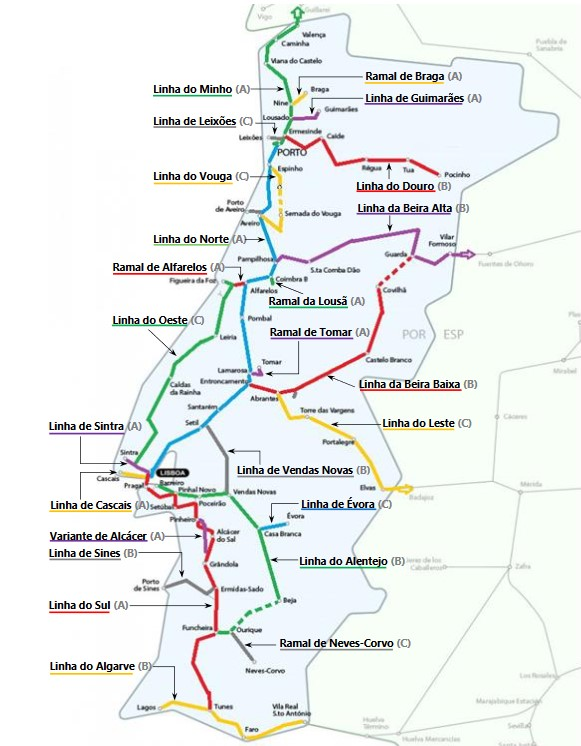
\includegraphics[scale = 0.5]{Figures/CPLines.jpg}
    \caption{Railway Network in usage in Portugal}
    \label{fig:CPLines}
\end{figure}

Passenger transport services are split into 3 main categories, Urban and Suburban transports, Inter-regional lines, and long-distance services namely \textit{Intercidades}, a medium speed solution, and \textit{Alfa-Pendular} lines, the high-speed Portuguese solution.

\begin{figure}[h]
    \centering
    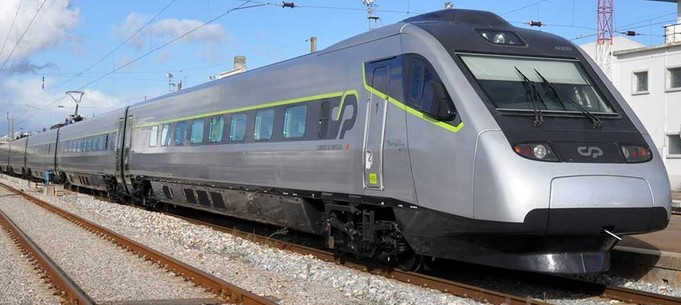
\includegraphics[scale =0.5]{Figures/Alfa.jpg}
    \caption{Portuguese High-Speed Train \textit{Alfa-Pendular}}
    \label{fig:Alfa}
\end{figure}

With a continuous increase in usage, the importance of the Portuguese railway services has been acknowledged by the central government, resulting in the creation of multiple programs for the update and continued electrification efforts of all lines.

In the following sections, the three most important lines will be detailed and the compositions that compose said lines will also be described in greater detail.

\subsection{Lisbon-Sintra Lines}
\subsection{Suburban Porto Line}
\subsection{\textit{Alfa-Pendular} Line}

\section{Electric motorization in use in rolling stock}\label{sec:sota_motor}
The best engine choice for electric locomotives varies wildly given both speed and torque requirements, as well as non-functional requirements like cost, cost of maintenance, and reliability.

A balance between both functional and non-functional parameters needs to be reached in order to correctly identify the best motor option to be implemented. 

To better understand the different motor types generally used in railway applications, this section will provide a detailed insight on the workings of each allowing a final evaluation and comparison of each motor typology.  
\subsection{Direct Current Motors}

Due to their low cost and ease of control, DC motors have historically been widely used for speed control applications like in an electric locomotive. 

However, due to their inherited operating principles, they require higher maintenance. This maintenance involves the replacement or treatment of the brushes and commutators that deteriorate during normal motor operations. 

\begin{figure}[ht]
    \centering
    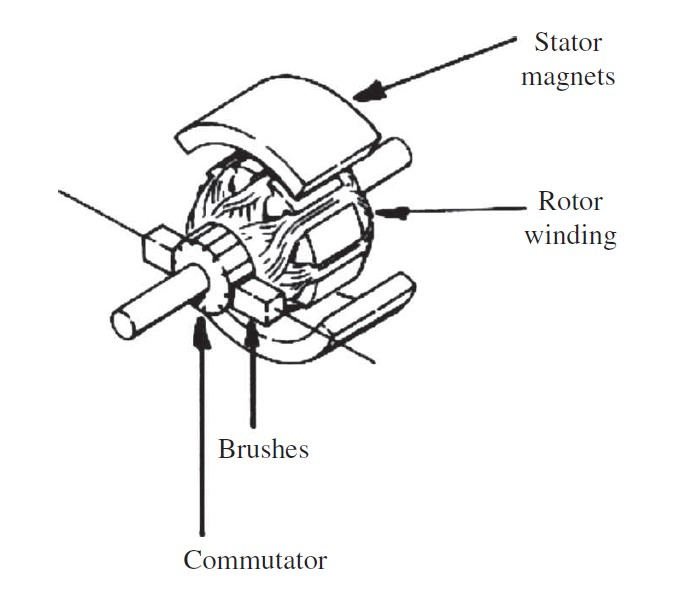
\includegraphics[scale = 0.5]{DC_MOTOR_Exploded.jpg}
    \caption{Construction of a DC Motor \cite{Mohan}}
    \label{fig:DC_Motor}
\end{figure}

The operating principles of DC machines are generally similar to any other electric machine. A coil usually located either in the rotor of the machine is supplied by a current that reverses polarity in every half-cycle creating a magnetic field that also reverses the polarity every half-cycle \cite{Mohan}. From the interaction of the magnetic field generated in the rotor and the already present magnetic field of the stator (typically caused by permanent magnets,\ref{fig:DC_Motor}) a varied magnetic field is generated in the air gap between the stator and rotor provoking a torque in the shaft of the motor. 

The reversal of current in the rotor is done using the aforementioned commutator and brushes that need to be in constant contact during the rotation of the engine causing the wear mentioned earlier.

Compared to other typologies, the price of DC motors increases with the power of the motor at a much higher rate. This combined with the maintenance costs and advancements in semi-conductor technologies, which will be mentioned later in this section, led to the phasing out of these types of engines in most medium to high-speed railway locomotives.

\subsection{Induction Motors}
Due to their low cost, low maintenance requirements, and ease of control when compared to other AC motors, induction motors (IM's) have become the most used motor type in railway applications \cite{MainSOTA}. As such special attention will be given to the operation and construction of these types of motors. 

IMs can have several details in their construction. In general, for high power applications such as electric locomotives, IMs use squirrel cage, \ref{fig:SquirrelCage}, type rotor used to reduce ferromagnetic losses due to magnetic field interactions. 
\begin{figure}[ht]
    \centering
    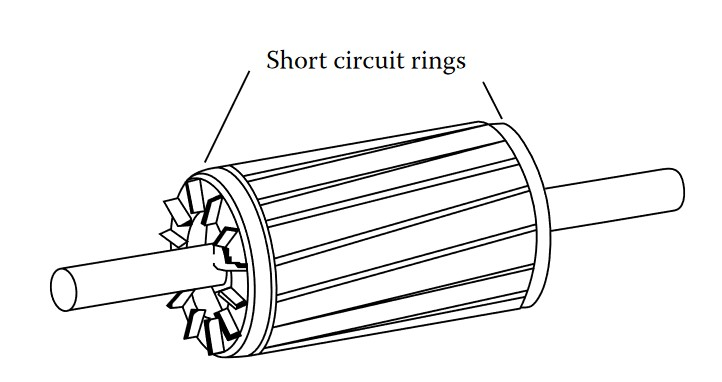
\includegraphics[scale = 0.5]{Figures/RotorSquirrleCageIM.jpg}
    \caption{Illustration of a squirrel cage rotor \cite{BibBase}}
    \label{fig:SquirrelCage}
\end{figure}
\subsubsection{Working principals of an induction motor}
As a general overview, IMs are composed of an inductor, usually located in the stator, and an inductee, usually located in the rotor. 

As the inductor windings are traversed by a varied current a varied magnetic field is created. This magnetic field, as it overlaps with the inductee windings, induces an E.M.F (electromotive force) that in turn generates a current creating another magnetic field that opposes the one created in the inductor. 

The interaction between these two fields creates torque in the shaft of the motor.

Now in detail, let's start by considering a rotor where the windings are not shorted. We can define the magnetic flux created in the stator as:
\begin{equation}\label{StatorFlux}
    \Phi = \frac{E_s}{k_s\*\omega_s}
\end{equation}

Where $k_s$ is a constant that translates the number of winding, construction of the stator windings, etc.

When the flux $\Phi$ crosses the rotor windings it creates an E.M.F. in the rotor such that:
\begin{equation}
    E_r = k_r\*\Phi\*\omega_r
\end{equation}

Where $k_r$ is a constant that translates the number of winding, construction of the rotor windings, etc.

$\omega_r$ represents the angular velocity of all rotor quantities. Remembering that the rotor can be mechanically spinning, $\omega_m$ - mechanical angular velocity, we can characterize $\omega_r$ as:

\begin{equation}
    \omega_r = \omega_s - \omega_m
\end{equation}

The value of $\omega_r$ is generally discussed as the absolute slip of the machine, i.e. the difference between the flux's angular velocity and the mechanical rotation of the motor axis. This is why IMs are described as asynchronous.

The slip, $s$, is usually presented as a relative measure:
\begin{equation}
    s = \frac{\omega_s-\omega_m}{\omega_s}
\end{equation}

To better understand the concepts above, and considering now a short-circuited rotor, an electric schema of the motor is presented below:
\begin{figure}[ht]
    \centering
    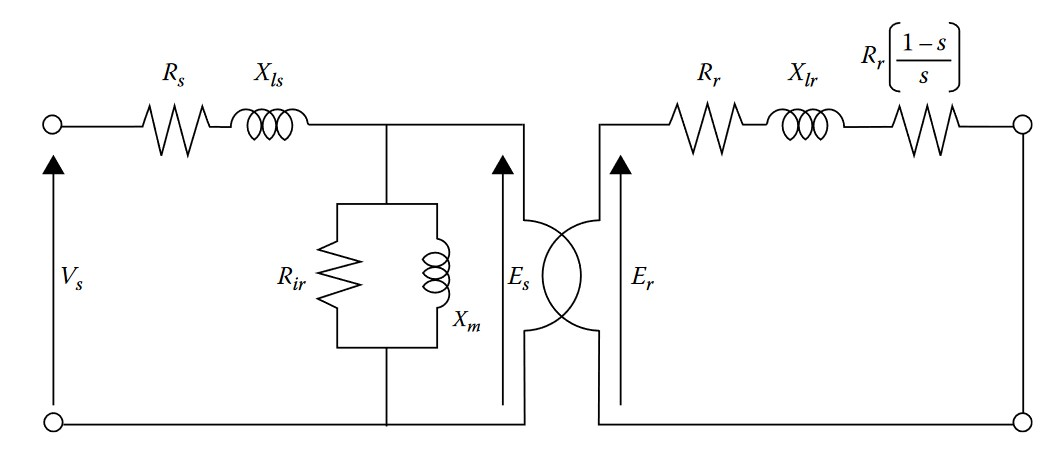
\includegraphics[scale = 0.45]{Figures/InductionMotorEquiv.jpg}
    \caption{IM Equivalent Circuit \cite{BibBase}}
    \label{fig:my_label}
\end{figure}

Where $R_r\frac{1-s}{s}$ represents the total mechanical load placed in the motor axle.
From the analysis of the equivalent circuit, we can determine that the mechanical power delivered by the motor is equal to:
\begin{equation}\label{MecPower}
    P_m = 3\*R_r\*I_r^2\*\frac{1-s}{s}
\end{equation}

From this, \ref{MecPower}, the mechanical torque generated can be described as:
\begin{equation}
    T_m = \frac{P_m}{\omega_r} = \frac{3\*R_r\*I_r^2}{s\*\omega_s}
\end{equation}

As a function of stator current and voltage, $I_r$ can be described as follows:
\begin{equation}
    I_r(I_s,V_s) = 
\end{equation}

Thusly the general control of the torque and by the effect the velocity of the axle can be described as a combination of the previous equations.

Although the slip induced in IMs augments the complexity of vector control techniques for IMs, it provides the machine with an inherit means to support changes of speed in the rotor without needing to specifically determine the appropriate current for each load variation. This is particularly helpful in railway applications eliminating the necessity for individual control of each axis during cornering \cite{MainSOTA}.

The slip also allows for the bulk control of several engines by a single converter, reducing implementation costs and control complexity \cite{Motor-SOTA}.

\subsection{Permanent Magnet Synchronous Motors}
PMSMs notably have a higher torque density and much higher efficiency compared with induction motors as such, since 2005 \cite{Motor-SOTA}, efforts have been made in an attempt to implement permanent magnet motors in railway systems as a replacement for IM. However, due to the cost of rare earth elements used in the manufacturing of magnets the adoption of these types of motors has been limited \cite{MainSOTA}.

As the name implies, PMSMs use permanent magnets as a way to create a magnetic field that can interact with the one created by excitation of the windings by an alternating current. The remainder of the acronym  translates the synchronous nature of the motor, i.e. the rotor spins at the same frequency as the magnetic field created.

The fact that rotor frequency is equal to the magnetic field frequency introduces additional complexity to the control of these types of motors. As the speed of the motor is necessarily controlled by the frequency provided by the control it prohibits group drive of synchronous motors.\cite{MainSOTA},\cite{Motor-SOTA}. 

Safety concerns also due to the synchronous nature of these motor types implicates the addition of complex control systems in several components as brakes increase again the general cost of implementing synchronous motors \cite{Motor-SOTA}.

\subsection{Synchronous Reluctance Motors}
As the main candidate for the replacement of IM in railway applications, SynRMs have been the target of multiple efforts in recent years to be implemented in railway applications. Being, as of the time of writing, the most recent technology to be evaluated no trains in service are currently using SynRMs \cite{Motor-SOTA}.

Having a torque density comparable to PMSMs and an efficiency equally high, SynRMs have an edge over PMSMs over the costs. As previously discussed PMSMs vary widely in price due to the rare-earth metals needed in their construction, SynRMs are not constrained by such prices \cite{MainSOTA}.

However, SynRMs have a much higher control complexity and questions have been pointed regarding the mechanical strength of the rotor and the very low power factor \cite{Motor-SOTA}.

\subsection{Comparison and Evaluation}
Throughout the railway industry, the motorization is selected by a balance of the price of the solution for the necessary load, reliability, controllability, efficiency, torque density, and maximum speed, plus a multitude of other measurements of the possible solution that are specific to each application. In general, however, we can evaluate the efficacy of each motor typology for a general railway system. The following table was created \cite{MainSOTA} using a 5 scale evaluation of each parameter described. 

\begin{table}[ht]

    \centering
    \caption{Evaluation of traction motors available and implemented in rolling stock solutions}
    \begin{tabular}{c|c c c c}
        \hline\hline
        Parameters     & DC & IM & PMSM & SynRM \\
        \hline
         Cost & 4 & 5 & 3 & 4.5\\
         Reliability & 2 & 4.5 & 4 & 5\\
         Controllability & 5 & 5 & 4 & 3.5\\
         Efficiency & 3.5 & 3.5 & 5 & 4\\
         Torque Density & 3 & 3.5 & 5 & 4\\
         Maximum Speed & 3 & 5 & 3.5 & 4\\
         \hline
         $\sum $ Total & 20.5 & 27 & 23.5 & 25\\
         \hline\hline
    \end{tabular}
    
    \label{tab:MotorEval}
\end{table}

From \ref{tab:MotorEval}, we can conclude that generally, induction motors provide, in high-speed rail application and in fact most railway applications, the best option for motorization. Even so, the notable efficiency and torque density of PMSMs and SynRMs indicate that as these technologies advance we may see in the future several urban and suburban lines using these types of motors.


\section{Power supply options in railway applications} \label{PowerSup} 
Following the previous section, it is now relevant to discuss the way in which electrical power is delivered to the motors.

Generally, most railway services use overhead lines as a way to transport energy. Trains then use a system such as an overhead catenary to transfer said energy to the systems within the train.

Historically the distribution was done using DC. DC distributions still have a relevant market share throughout different railway services \cite{OldSota}. However,  the well-known problems with high losses caused by DC distribution and the increased complexity and cost of converting and injecting energy to and from an AC grid has led to the decrease in market share of this type of distribution.

Currently, most services use AC distribution with frequencies between 50 and 60 Hz. The voltage levels are varied and will be described in the following sub-section.

\subsection{Voltage Standards Around the World}
From information gathered form \cite{OldSota} and \cite{MainSOTA} the following schema was constructed to detail the varied voltage levels used in railway services.
\begin{figure}[ht]
    \centering
    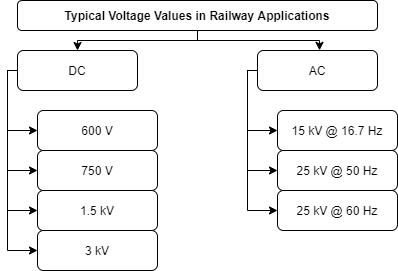
\includegraphics[scale = 0.5]{Figures/VoltageLevels.png}
    \caption{Voltage levels in use in railway power supply applications}
    \label{fig:Vlevels}
\end{figure}

As it can be seen from the schema \ref{fig:Vlevels} there is a multitude of levels and frequencies that increase the difficulty of creating plug-and-play solutions for converter technologies for railway services.

Now in detail to the Portuguese railway services, most of the electrified lines use a 25 kV @ 50Hz with a single overhead line. There is however a line, \textit{Liha de Cascais} that still uses 1.5 kV DC. 

The distribution is done using substations along the line that convert the energy from the main energy network to a correct voltage level. The substations are spaced in such a way that there is no interference between one another, this creates some zones where there is no power being supplied to the overhead line. This is usually not a problem but it is relevant to take into account when designing a complete system to be implemented.

The energy received by the train needs to be used to supply both the auxiliary systems and the motors and other primary systems that realize all the functions of the train. To be able to supply all the different systems the energy needs to be converted. In the next section, a general converter will be detailed paying special attention to the power being supplied to the driving systems.

\subsection{Generic Converter Schema}
The power received by the train needs to be appropriately conditioned and regimented in order to then be able to be used to supply not only the driving components but also for all auxiliary systems.

The use of transformers provides the ability to control the voltage level for all different systems. After the voltage levels are regulated to the required value, and focusing now on the driving components of the train, there is a necessity to convert the AC or DC power in order to drive the motor that is being supplied.

The building of a power system must also take into account the typology of the train. In general, there are two construction types of power systems, a concentrate configuration where there is a locomotive pushing or pulling the coaches and a distributed system where multiple units spread throughout the coaches powering multiple axes.

These two systems give origin to different electrical solutions when it comes to the design of the converter. In the sections below the varied schema will be described and exemplified comparing the advantages and disadvantages of each.
\subsubsection{Locomotive schema}
From the locomotive converter schema represented in \cite{} we can deduce that the cost of implementation may be reduced when in comparison to the EMUs the simplicity in control and electronic technologies creates a simpler more robust solution. 

However, this kind of typology creates the necessity for more power full motor and higher capacity electronics that can be limiting. For the same reason, in short-run applications such as suburban lines or even shorter urban or subway lines locomotive configurations are not ideal.

\subsubsection{EMU schema}
Recently and due to the increased capabilities of controllers, the implementation of EMUs has risen in recent years.

As the schema above shows the electric schema for the implementation of EMU includes more electronics and more sophisticated limiting and protection equipment. This increases the price of all power supply components. However and as it has been said earlier, EMUs allow for smaller more compact motors and a reduction in load from each individual converter.

\subsection{Evolution of Converter and Semi-Conductor Technology}
As it is expected the driving converters, i.e. the converters that supply the motors, are of enormous importance to the efficiency, reliability, and control-ability of the train. As such the technologies used in these are of major importance. 

Historically DC motors were controlled using diode rectifiers with tap control or later with phase-controlled thyristors.
AC machines, either synchronous or asynchronous, began to be controlled using gate turn-off thyristors. 

Most modern lines are now using insulated gate bipolar transistors and some trials have begun using silicon carbide technologies in order to reduce losses and increase switching frequency.

In the next sections, each technology will be detailed and finally, a comparison will be done between the different technologies.

\subsubsection{Diodes and thyristors (Gate Turn-Off thyristors)}
The most simple and older of the technologies detailed in this segment, diodes are built using the simple combination of a P-N junction. The use of these allowed for passive speed control of DC motors as they can control the amount of energy released from the power supply.

Thyristors are an advancement on the technologies that built diodes, these can be controlled and inhibit the current flowing through them from an external gate.
\subsubsection{Insulated Gate Bipolar Transistors}
Insulated gate bipolar transistors are an hybrid with a MOS similar gate and a driven part closely related with a bipolar transistor (i.e. a p-n-p or n-p-n junction). From the construction of these types of transistors a diode naturally appears has a result of the junctions created. 

The use of IGBT increased since their creation in the 1980s and allowed for the increased in switching frequency, creating better harmonic compositions, a reduction in weight and volume allowing for more compact drives, and a reduction in losses due to the decreasing resistance in conduction. 

Using data gathered in \cite{MainSOTA} a comparison can be done between GTOs and IGBTs as it can be seen in \ref{fig:GTOvIGBT}.

\begin{figure}[h]
    \centering
    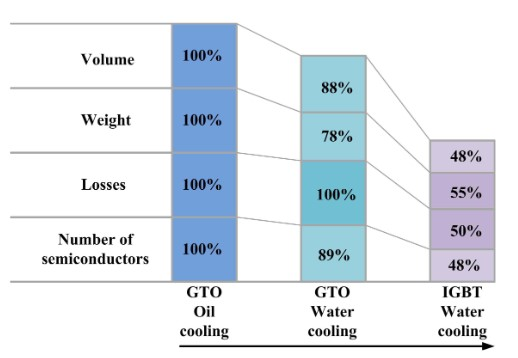
\includegraphics{Figures/IGBTvGTO.jpg}
    \caption{Comparison between IGBTs and GTOs \cite{MainSOTA}}
    \label{fig:GTOvIGBT}
\end{figure}

\subsubsection{Silicon Carbide and Hybrid Power Semi-Conductors}
The future technologies to note regarding semi-conductors are without any doubt the usage of silicon carbide (SiC), gallium semi-conductor or an hybrid combination of regular IGBT construction and SiC.

With the support of several state programs and with a rapid increase in capability, the implementation of SiC in railway applications is pointed as a requirement for any future converters to be implemented put into rolling stock.

SiC technologies provide an even greater reduction in volume and weight when compared to IGBTs and greater switching frequencies. 

The most evolved and tested usage of SiC in power electronics is the implementation in SiC of the Shottky diode in a regular silicon based IGBT. This brings the advantage of reducing recovery and turn-off losses caused by the switching of the built-in diode. It also reduces turn-on and conduction losses but to a lesser degree. 

Experimentation of these technologies are already under way in Japanese rail with great success reducing by 35\% inverter losses\cite{MainSOTA}.

\begin{figure}[h]
    \centering
    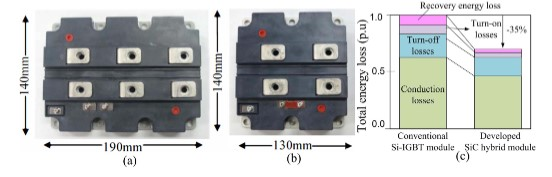
\includegraphics{Figures/SivSiC.jpg}
    \caption{Comparison(c) between Si-IGBT(a) modules and SiC hybrid modules(b)}
    \label{fig:SiVSiC}
\end{figure}

\section{Control techniques of AC electric motors}
In AC motor control one can relate the speed and torque of the motor as a relationship between the amplitude of the voltage or current delivered and the frequency of the signal. The changing of the two in way to provide the desired speed or torque is the ultimate goal of any controller.

In this section, higher relevance will be given to the control of IM as these are the most widely used and the type of machine that will be discussed and used in the following chapters of this dissertation.

\subsection{Voltage over Frequency Speed Control}
The oldest and most used control techniques of IMs are scalar methods which utilize a steady-state model of the motor in order to rework the frequency and amplitude of the supply. This results in very poor control dynamics. 

One of the most used scalar control methods is voltage over frequency control. This control technique, sometimes used in open-loop, alters both the frequency and amplitude of the supply but maintaining the ratio between the two.\cite{BibBase}

This methodology has many drawbacks when in use throughout the full range of speed of the train. At low velocities the low switching frequency results in high losses and low controllability whilst at high speeds the drawbacks are lower there is still the same problem of an increased switching frequency and the influence of poor dynamics is even more noticeable.\cite{ScalarSOTA}

Regarding what is described in \cite{ScalarSOTA} the prevalence of scalar methods for low computation and low dynamic control in combination with more sophisticated methods such as field oriented control is reasonable and very much usable. Although the evolution and advancements in computation and complex vector controllers is without a doubt the future of traction control technologies.

Bellow is represented a schematic of the closed loop implementation of V/f control.

\subsection{Vector Control Techniques}
To understand vector control we must first talk about the vector transformations that allow the three-phase sinusoidal values of AC electrical machines to two orthogonal vectors with DC amplitudes.

\begin{figure}[h]
    \centering
    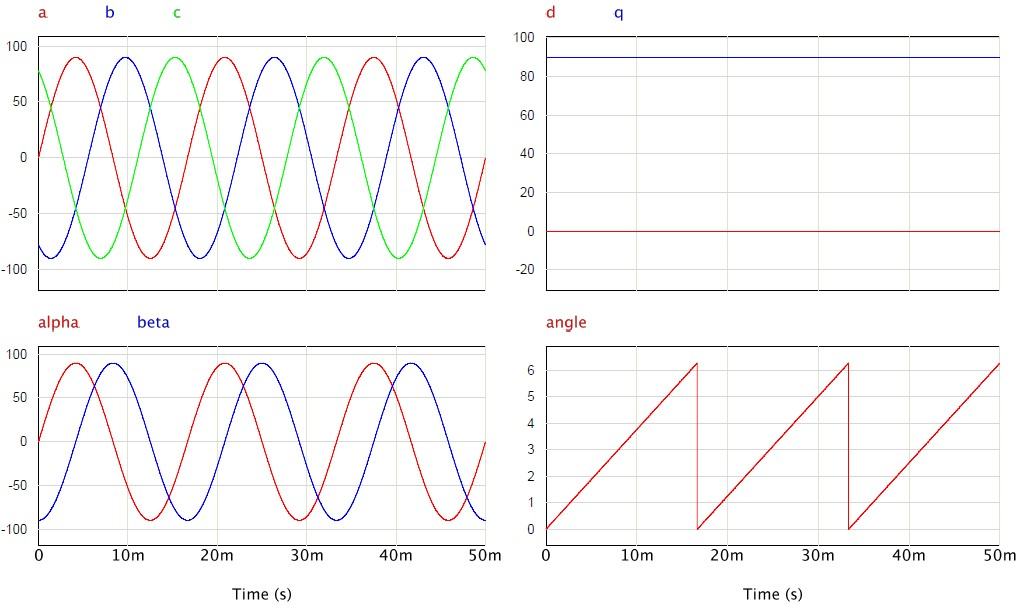
\includegraphics[scale = 0.5]{Figures/ClarkPark.jpg}
    \caption{Clark-Park transform visualization: a,b,c 3 phase sinusoidal supply (top left); Clark transformation result (bottom left); Park transform result (top right); Angle of rotation used in Park transform (bottom right)}
    \label{fig:albet-dq0}
\end{figure}

The transformations that allow for this conversion are the Clark-Park transforms. This transformation starts by representing the 3 phase reference frame as a 2 phase orthogonal reference frame (Clark transformation).

\begin{equation}
    x_{\alpha \beta \gamma} = \frac{2}{3}\begin{bmatrix}
1 & -1/2 & -1/2 \\
0 & \sqrt{3}/2 & -\sqrt{3}/2 \\
1/2 & 1/2 & 1/2
\end{bmatrix}x_{abc}
\end{equation}

The resulting values from this transform are still sinusoidal values. To obtain the DC value vectors the 2 phase orthogonal frame created by the Clark transform can rotate at the frequency of the previous values. This results in two orthogonal vectors with DC values.
\begin{equation}
    x_{dq0} = \begin{bmatrix}
    cos(\theta) & sin(\theta) & 0 \\
    -sin(\theta) & cos(\theta) & 0\\
    0 & 0 & 1 \\
    \end{bmatrix}x_{\alpha\beta\gamma}
\end{equation}

The nature of the values allows for traditional control techniques, such as PI controllers, can more easily be used giving the ability to create more precise control techniques.

From the application of the full Clark-Park transformation to the currents of an IM machine, we can relate $I_d$ as the vector responsible for the creation of flux and $I_q$ as the current vector responsible for torque creation. From this several control, techniques can be designed.

\subsubsection{Field Oriented Control}
Field oriented control (FOC) utilizes the separation described above between the current that generates torque and the current that generates the necessary magnetic field. From this separation FOC utilizes a reference value in speed or torque or a current value for $I_q$ current and separately a reference for $I_d$ current is calculated such that the magnetic field generated is equal to the nominal field that is required.

After the calculations done in FOC the required currents $I_d$ and $I_q$ must be resolved into the commands for the inverter. This is achieved through modulation. The most widely used and considered modulation technique is space-vector modulation (SVM). SVM uses a set of vectors that represent the voltages obtained from the different combinations of the inverter. The use of modulations enables the switching frequency to be constant throughout the range of working velocities of the motor.

As in all of the following traction techniques FOC can be implemented from many different sub-techniques. The simplest and better described version of field oriented control is DFOC (direct field oriented control) where the speed and stator currents of the motor are measured resulting in almost direct implementation from the values obtained from the motor to the control algorithms. 

The other relevant specification of FOC is IFOC (indirect field oriented control), has the name implies IFOC estimates the speed of the motor from the stator currents measured. This increases the in-dependability from motor parameters and reduces the cost and amount of equipment used in the control mesh.

Comparing IFOC to DFOC it can be said that DFOC as good dynamic control above nomnal speeds and is easier to implement when compared to IFOC. IFOC is better suited for bellow nominal speed ranges in which sensor reading are less accurate, however the implementation of IFOC is more complex and is less robust in terms of system security being only reliant on an online estimation of the speed of the rotor \cite{DFOC-IFOC}. 

With any of these typologies different ad-ons can be implemented in order to improve the characteristics of each. For example, the common problem of parameter dependence encountered in DFOC can be reduced using online parameter estimation better relating the nominal values used in simple DFOC to the real values that would be measured during motor operations.

The improvement of IFOC with the use of both parameter estimation and model representative adaptive control can also lead to a better more reliable system relating the real working parameters of the motor with the nominal values used in both speed estimation blocks and fine-tuning of all PI controllers.

Comparing the complexity and advantages of both DFOC and IFOC for railway applications it was identified that DFOC with parameter estimation was the most useful control system since it reduces the downside of parameter dependence inherit to DFOC while also providing better nominal speed dynamics which are more relevant to high speed railway applications when compared to IFOC.

There, however, other common control techniques that should be considered for control of IM. As such the next sections will describe the upsides and downsides of other control methodologies that can be implemented in these systems.
\subsubsection{Direct Torque Control}
DTC was implemented as a simplification of FOC, eliminating the necessity for current controller as implemented in FOC and directly control rotor flux and torque from the values estimated. The general idea of DTC is to implement a look-up table that has been experimentally obtained that uses the estimated torque and rotor flux to determine which voltage vectors need to be active within the inverter. This eliminates the necessity for modulation within the control mesh further reducing the complexity of the control technique. 

DTC is also an hysteresis control technique using hysteresis controllers to minimize the error between the reference values and the measured values.

As it stands, the benefits of DTC control are the reduction of complexity and cost to the control mesh. This however isn't without downsides. Mainly the variable switching frequency caused by the lack of modulation causes increasing instability to the inverter at both ends of the speed ranges also causing more unstable and unpredictable harmonic content. The usage of hysteresis controllers also increase the torque ripple due to the inherit non continuity of the controllers. 

Similarly to FOC DTC can also be implemented with different sub-types. The most used and most useful is the implementation of DTC with SVM (Space Vector Modulation). The usage of a modulation block as a substitute to the look-up table allows for a constant switching frequency and as such a much more predictable and  clean harmonic content. This is achievable through the use of empty or non-valued vectors through the points where there is no need to change the value of the voltage vector. Even thought the use of SVM the ripple problem introduced through the hysteresis controllers are maintained. 

Given the torque ripple created and the speed control abilities of this typology and the increasing capabilities of the micro-controllers diminished the advantage of these type of controller in this application.


\subsubsection{Model Predictive Control}

As the most advanced and progressive control method MPC uses a predictive model of the system, inverter and motor, using as inputs typical motor parameters such as speed, current measurements or torque to estimate what will be the next state of the system. The reference state and the predicted state are then feed to a cost function in order to determine the most efficient voltage vector to be order to the inverter. As such typical MPC controllers do not utilize any modulation techniques. 

Continuing the trend set by all other control techniques, MPC is also used in several different combinations. It is typical the usage of MPC with DTC combining the the ease of implementation of DTC with the enhanced efficiency and performance given by the cost functions determined by the MPC. The of SVM to fix the switching frequency also results in a different tyoe of MPC control which is simply called continuous control set MPC as it does no make use of the finite converter possibilities determined by the inverter. 

MPC has the advantage of simplifying the implementation and testing of non linear controllers and providing improvements to DTC which as led to an increased interest for railway applications. However the weights that factor into the cost function have no deterministic methods for their calculation, increasing the difficulty of implementing this control technique. The parameter influence and variable frequency provided by pure MPC-DTC diminish the usability of this control technique in any application.

\subsubsection{Comparison between different control methodologies}
Using information gathered from \cite{MainSOTA} and condensing information from the remaining sources mentioned earlier the following table was compressed.

\section{Anti-Slip Technologies}
Besides the main functions of a traction control system, there exists other problems brought up by the contact between the wheel and the rail. Mainly the reduction of the slip in breaking and acceleration operations can reduce both wear and increase safety and comfort within any application. 

Historically the problem of slip and detachment between the wheel and rail was handled using specific funnel with grit or sand that deployed it in front of the wheel increasing grip and stability. This deployment was done manually by the conductor. 

More recently and given the advancements in technologies and sensing in traction control systems more advanced and complex anti-slip methodologies have come up. The building idea of most methods can be separated in two section, the detection of  slip between the wheel and the rail, and the correction and regaining of adhesion method to limit the amount of slip.

In the next sections a short but detailed overview of these two different building blocks of anti-slip technologies will be provided.
\subsection{Slip-detection}
\subsection{Re-adhesion techniques}

\section{European Train Control Systems and Guiding Norms and Regulations}
As mentioned previously the increased importance of railway both nationally and internationally between European countries as lead to an increased desire of creating an European standard grid and standard communication protocols. The increased opportunities to implement within the control schema of trains vision systems and other communication between trains as lead the European Union to create a gathering of capability levels that traction systems should follow.

The increased safety and security concerns come accompanied by a multitude of norms and regulation that should be of interest to any project developed in this area.

\subsection{ETCS levels}
The result of a consortium o companies interested in the development and implementation of tracion control systems for railway applications.
\subsection{Notable UIC norms}


\include{Chapters/chapter3}
\include{Chapters/chapter4}
\include{Chapters/chapter5} 

%% Comment next 2 commands if numbered appendices are not used
\appendix
\include{Aux/appendix1}

%%----------------------------------------
%% Final materials
%%----------------------------------------

%% Bibliography
%% Comment the next command if BibTeX file not used, 
%% Assumes that bibliography is in ``myrefs.bib''
\PrintBib{myrefs}

%% Index
%% Uncomment next command if index is required, 
%% don't forget to run ``makeindex tese'' command
%\PrintIndex

\end{document}
